\documentclass{article}

\usepackage{fancyhdr} % Required for custom headers
\usepackage{lastpage} % Required to determine the last page for the footer
\usepackage{extramarks} % Required for headers and footers
\usepackage[usenames,dvipsnames]{color} % Required for custom colors
\usepackage{graphicx} % Required to insert images
\usepackage{listings} % Required for insertion of code
\usepackage{courier} % Required for the courier font
\usepackage{lipsum} % Used for inserting dummy 'Lorem ipsum' text into the template
\usepackage{amsmath}
\usepackage{amssymb}
\usepackage{mathtools, xparse}
\usepackage{booktabs}
\usepackage{bigstrut}
\usepackage{float}
\usepackage{hyperref}
\usepackage{color}
\usepackage{algorithm}
\usepackage{caption}
\captionsetup{skip=0pt}
\usepackage{algpseudocode}
\usepackage{multirow}
\usepackage{subfigure}
\usepackage{longtable}
\usepackage{supertabular}
\usepackage{biblatex}

\renewcommand*{\Rnfont}{\scshape}

\DeclarePairedDelimiter{\norm}{\lVert}{\rVert}
\DeclarePairedDelimiter\abs{\lvert}{\rvert}%

\hypersetup{
    colorlinks   = true,    % Colours links instead of ugly boxes
    urlcolor     = red,    % Colour for external hyperlinks
    linkcolor    = red,    % Colour of internal links
    citecolor    = red      % Colour of citations
}
% Margins
\topmargin=-0.45in
\evensidemargin=0in
\oddsidemargin=0in
\textwidth=6.5in
\textheight=9.0in
\headsep=0.25in

\linespread{1.1} % Line spacing

% Set up the header and footer
\pagestyle{fancy}
\lhead{\hmwkAuthorName} % Top left header
\rhead{\hmwkClass\ : \hmwkID} % Top center head
%\rhead{\firstxmark} % Top right header
\lfoot{\lastxmark} % Bottom left footer
\cfoot{} % Bottom center footer
\rfoot{Page\ \thepage\ of\ \protect\pageref*{LastPage}} % Bottom right footer
\renewcommand\headrulewidth{0.4pt} % Size of the header rule
\renewcommand\footrulewidth{0.4pt} % Size of the footer rule
\renewcommand{\subsectionmark}[1]{\markboth{#1}{}}
\setlength\parindent{0pt} % Removes all indentation from paragraphs

%----------------------------------------------------------------------------------------
%	CODE INCLUSION CONFIGURATION
%----------------------------------------------------------------------------------------

\definecolor{MyDarkGreen}{rgb}{0.0,0.4,0.0} % This is the color used for comments
\lstloadlanguages{Perl} % Load Perl syntax for listings, for a list of other languages supported see: ftp://ftp.tex.ac.uk/tex-archive/macros/latex/contrib/listings/listings.pdf
\lstset{language=Perl, % Use Perl in this example
    frame=single, % Single frame around code
    basicstyle=\small\ttfamily, % Use small true type font
    keywordstyle=[1]\color{Blue}\bf, % Perl functions bold and blue
    keywordstyle=[2]\color{Purple}, % Perl function arguments purple
    keywordstyle=[3]\color{Blue}\underbar, % Custom functions underlined and blue
    identifierstyle=, % Nothing special about identifiers                                         
    commentstyle=\usefont{T1}{pcr}{m}{sl}\color{MyDarkGreen}\small, % Comments small dark green courier font
    stringstyle=\color{Purple}, % Strings are purple
    showstringspaces=false, % Don't put marks in string spaces
    tabsize=5, % 5 spaces per tab
    %
    % Put standard Perl functions not included in the default language here
    morekeywords={rand},
    %
    % Put Perl function parameters here
    morekeywords=[2]{on, off, interp},
    %
    % Put user defined functions here
    morekeywords=[3]{test},
    %
    morecomment=[l][\color{Blue}]{...}, % Line continuation (...) like blue comment
    numbers=left, % Line numbers on left
    firstnumber=1, % Line numbers start with line 1
    numberstyle=\tiny\color{Blue}, % Line numbers are blue and small
    stepnumber=5 % Line numbers go in steps of 5
}

% Creates a new command to include a perl script, the first parameter is the filename of the script (without .pl), the second parameter is the caption
\newcommand{\perlscript}[2]{
    \begin{itemize}
        \item[]\lstinputlisting[caption=#2,label=#1]{#1.py}
    \end{itemize}
}
\newcommand{\cppscript}[1]{
    \begin{itemize}
        \item[]\lstinputlisting[]{#1}
    \end{itemize}
}

%----------------------------------------------------------------------------------------
%	DOCUMENT STRUCTURE COMMANDS
%	Skip this unless you know what you're doing
%----------------------------------------------------------------------------------------

% Header and footer for when a page split occurs within a problem environment
\newcommand{\enterProblemHeader}[1]{
    \nobreak\extramarks{#1}{#1 continued on next page\ldots}\nobreak
    \nobreak\extramarks{#1 (continued)}{#1 continued on next page\ldots}\nobreak
}

% Header and footer for when a page split occurs between problem environments
\newcommand{\exitProblemHeader}[1]{
    \nobreak\extramarks{#1 (continued)}{#1 continued on next page\ldots}\nobreak
    \nobreak\extramarks{#1}{}\nobreak
}

%\setcounter{secnumdepth}{0} % Removes default section numbers
\newcounter{homeworkProblemCounter} % Creates a counter to keep track of the number of problems

\newcommand{\homeworkProblemName}{}
\newenvironment{homeworkProblem}[1][Problem \arabic{homeworkProblemCounter}]{ % Makes a new environment called homeworkProblem which takes 1 argument (custom name) but the default is "Problem #"
    \stepcounter{homeworkProblemCounter} % Increase counter for number of problems
    \renewcommand{\homeworkProblemName}{#1} % Assign \homeworkProblemName the name of the problem
    \section{\homeworkProblemName} % Make a section in the document with the custom problem count
    \enterProblemHeader{\homeworkProblemName} % Header and footer within the environment
    }{
    \exitProblemHeader{\homeworkProblemName} % Header and footer after the environment
}

\newcommand{\problemAnswer}[1]{ % Defines the problem answer command with the content as the only argument
\noindent\framebox[\columnwidth][c]{\begin{minipage}{0.98\columnwidth}#1\end{minipage}} % Makes the box around the problem answer and puts the content inside
}

\newcommand{\homeworkSectionName}{}
\newenvironment{homeworkSection}[1]{ % New environment for sections within homework problems, takes 1 argument - the name of the section
    \renewcommand{\homeworkSectionName}{#1} % Assign \homeworkSectionName to the name of the section from the environment argument
    \subsection{\homeworkSectionName} % Make a subsection with the custom name of the subsection
    \enterProblemHeader{\homeworkProblemName\ [\homeworkSectionName]} % Header and footer within the environment
    }{
    \enterProblemHeader{\homeworkProblemName} % Header and footer after the environment
}

%----------------------------------------------------------------------------------------
%	NAME AND CLASS SECTION
%----------------------------------------------------------------------------------------

\newcommand{\hmwkID}{hw03} % Assignment title
\newcommand{\hmwkTitle}{Photoacoustic Depth Profiling and SO2 Measurement}
\newcommand{\hmwkDueDate}{Tuesday,\ Dec\ 12,\ 2017} % Due date
\newcommand{\hmwkClass}{Principles of Biomedical Ultrasound and Photoacoustics} % Course/class
\newcommand{\hmwkClassTime}{10:30am} % Class/lecture time
\newcommand{\hmwkClassInstructor}{Jones} % Teacher/lecturer
\newcommand{\hmwkAuthorName}{106061531 Fu-En Wang} % Your name

%----------------------------------------------------------------------------------------
%	TITLE PAGE
%----------------------------------------------------------------------------------------

\title{
    \vspace{2in}
    \textmd{\textbf{\hmwkClass}}\\
    \textmd{\textbf{\hmwkID: \hmwkTitle}} \\
    \normalsize\vspace{0.1in}\small{Due\ on\ \hmwkDueDate}\\
    \vspace{3in}
}

\author{\textbf{\hmwkAuthorName}}
\date{} % Insert date here if you want it to appear below your name

%----------------------------------------------------------------------------------------

\begin{document}
\maketitle
\newpage

%\renewcommand\thesubsection{\thesection.\alph{subsection}}

\section{Part \RN{1}}
\subsection{Repeat Fig.1 in reference paper}
In the reference paper, they had simulated an acoustic wave of forward and backward wave. In this problem, we need to reproduce this
fig. Figure \ref{fig:p1a} shows the result.
\begin{figure}[H]
    \centering
    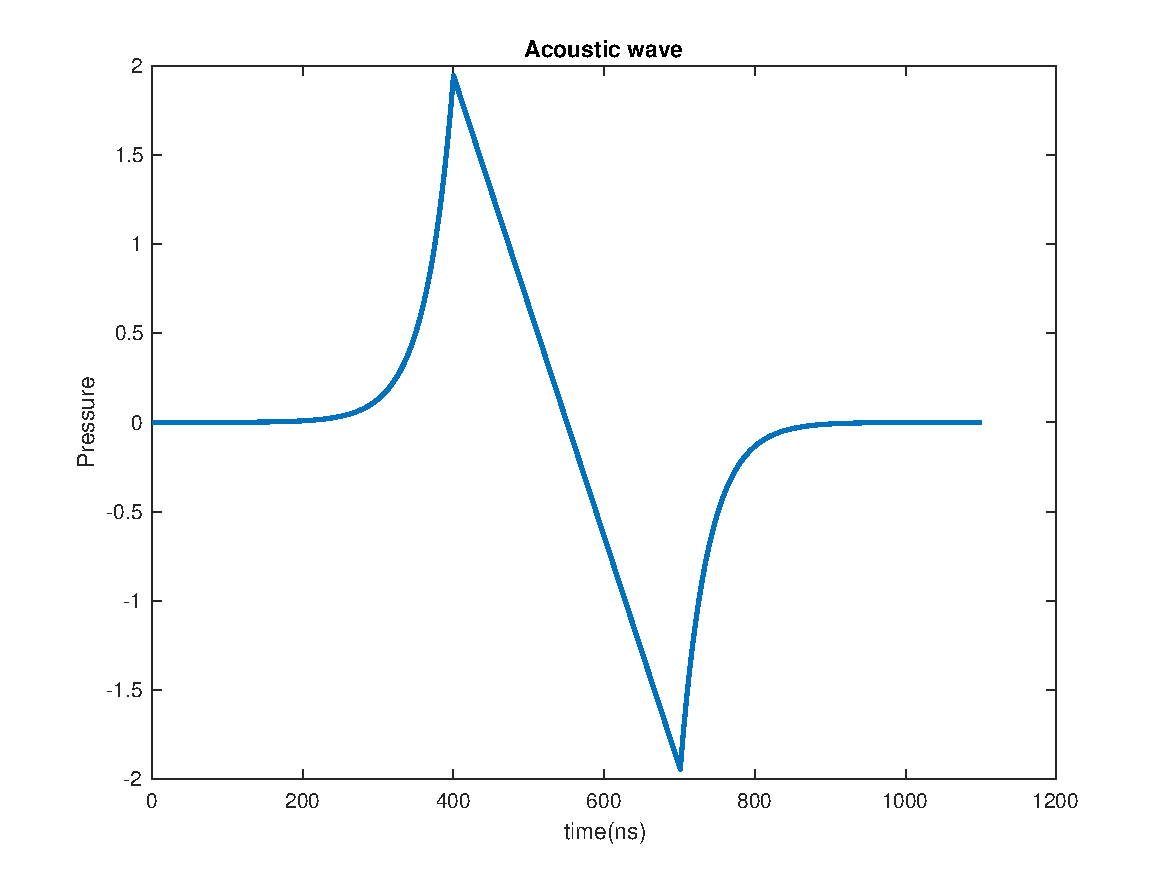
\includegraphics[width=0.7\textwidth]{src/p1a.pdf}
    \caption{Acoustic Wave}
    \label{fig:p1a}
\end{figure}
Because the part between positive and negative wave is implicit, I only use a straight line connecting the two peak points by 
dynamically solving a linear equation and make the space between them 300 ns.

\subsection{Repeat Fig.2 in reference paper}
Now add a gaussian noise to our signal which the ratio of standard deviation of the noise to the peak of the simulated 
photoacoustic signal is 5\%. Figure \ref{fig:p1b-1} shows the noisy signal and Figure \ref{fig:p1b-2} shows the exponential decay
of siganl.

\begin{figure}[H]
    \centering
    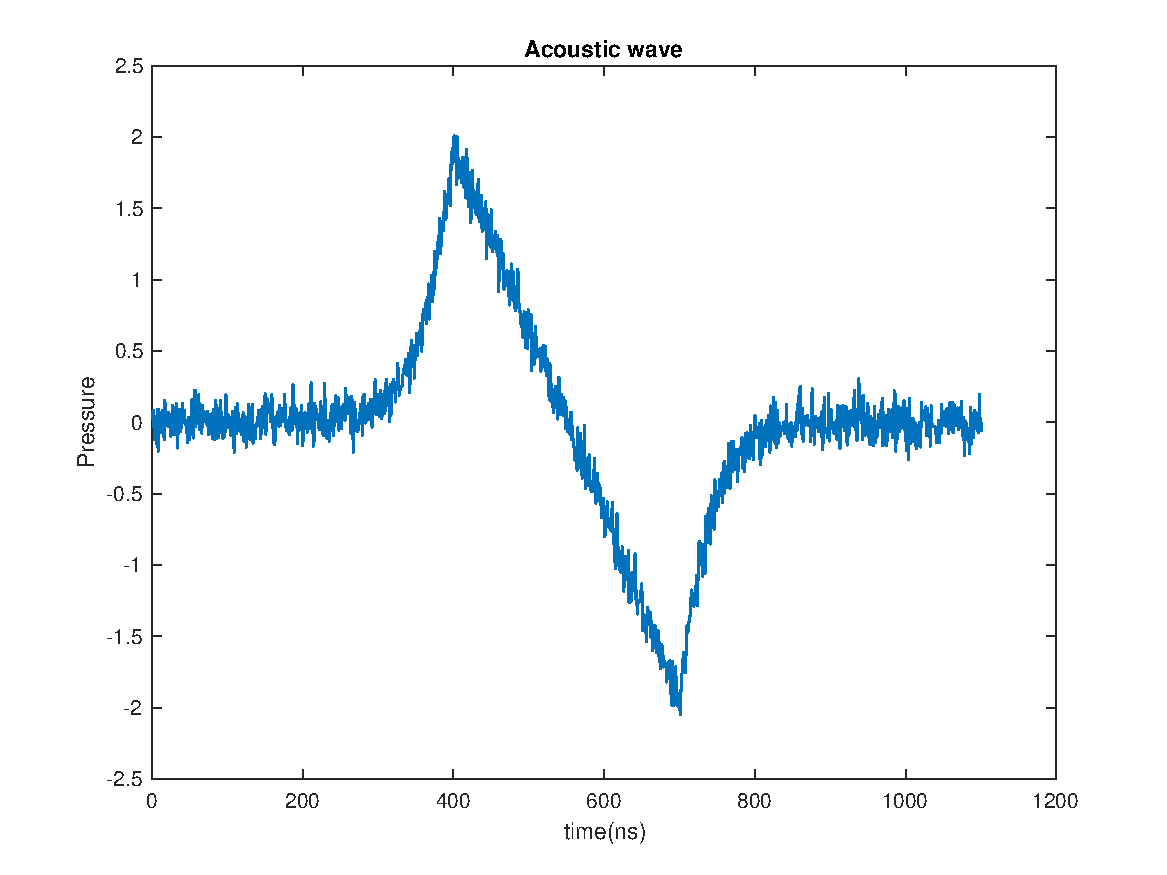
\includegraphics[width=0.7\textwidth]{src/p1b-1.pdf}
    \caption{Acoustic Wave with noise}
    \label{fig:p1b-1}
\end{figure}

In the reference paper, there is a equation for curve fitting this decay from author's experimental result.
$$
    p(z) = 9.5\exp^{-185z}
$$
Because the parameters I used is different, I adjust the amplitude from 9.5 to 1.94 as shown in Equation \ref{eq:decay}.
\begin{align}
    p(z) = 1.94\exp^{-185z}
    \label{eq:decay}
\end{align}
Now Figure \ref{fig:p1b-2} show the noisy decay and curve of Equation \ref{eq:decay}.

\begin{figure}[H]
    \centering
    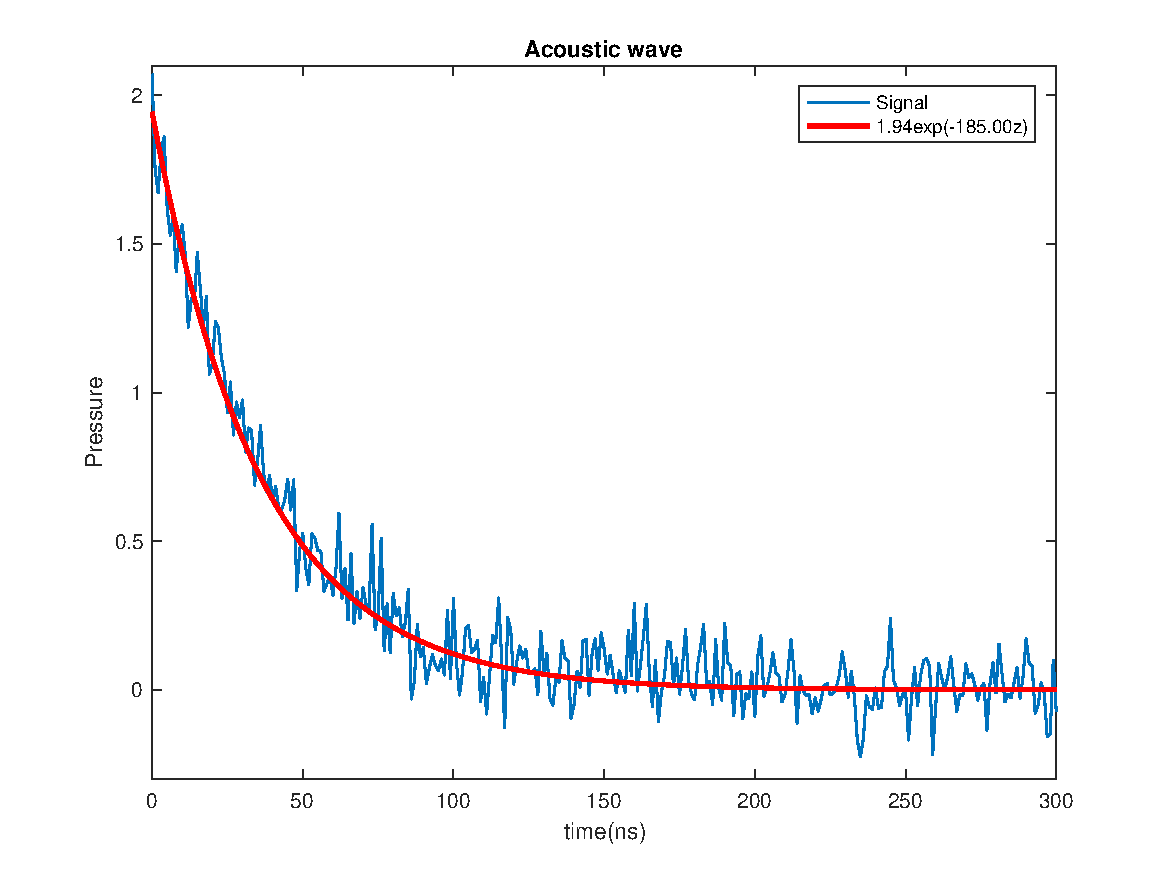
\includegraphics[width=0.7\textwidth]{src/p1b-2.pdf}
    \caption{Acoustic Wave with noise}
    \label{fig:p1b-2}
\end{figure}
In this figure, we can find that Equation \ref{eq:decay} is fitting well.


\subsection{Curve fitting for absorbtion coefficient}
Now from Figure \ref{fig:p1b-2}, we apply curve fitting and get our estimated $\mu_a$ of noisy signal. Figure \ref{fig:p1c} 
shows the estimated curve and noisy signal.

\begin{figure}[H]
    \centering
    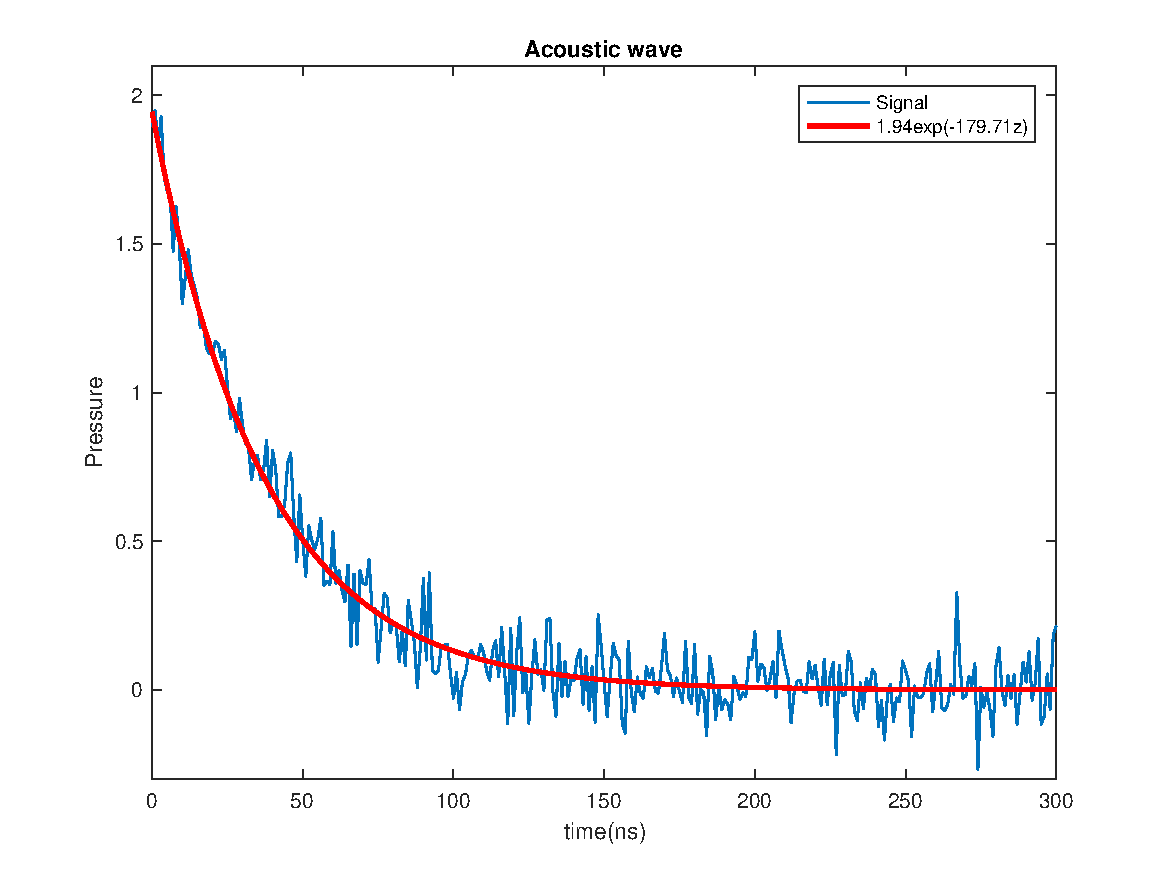
\includegraphics[width=0.7\textwidth]{src/p1c.pdf}
    \caption{Curve fitting for absorbtion coefficient}
    \label{fig:p1c}
\end{figure}

From my experimental result, the range of estimated $\mu_a$ is from 178 to 182 and the real $\mu_a$ I used is 180. 
As a result, the curve fits the signal pretty well I think.


\subsection{Peak value vs absorbtion coefficient}
\label{sec:p1d}
Theoretically, the peak of signal will proportional to $\mu_a$ which is $\mu_a \times \Gamma \times H_0 = 0.0108\mu_a$ in my case. 
so in this part, we need to plot the peak value of different absorbtion coefficient from 10 to 180. Figure \ref{fig:p1d} 
shows the result.
\begin{figure}[H]
    \centering
    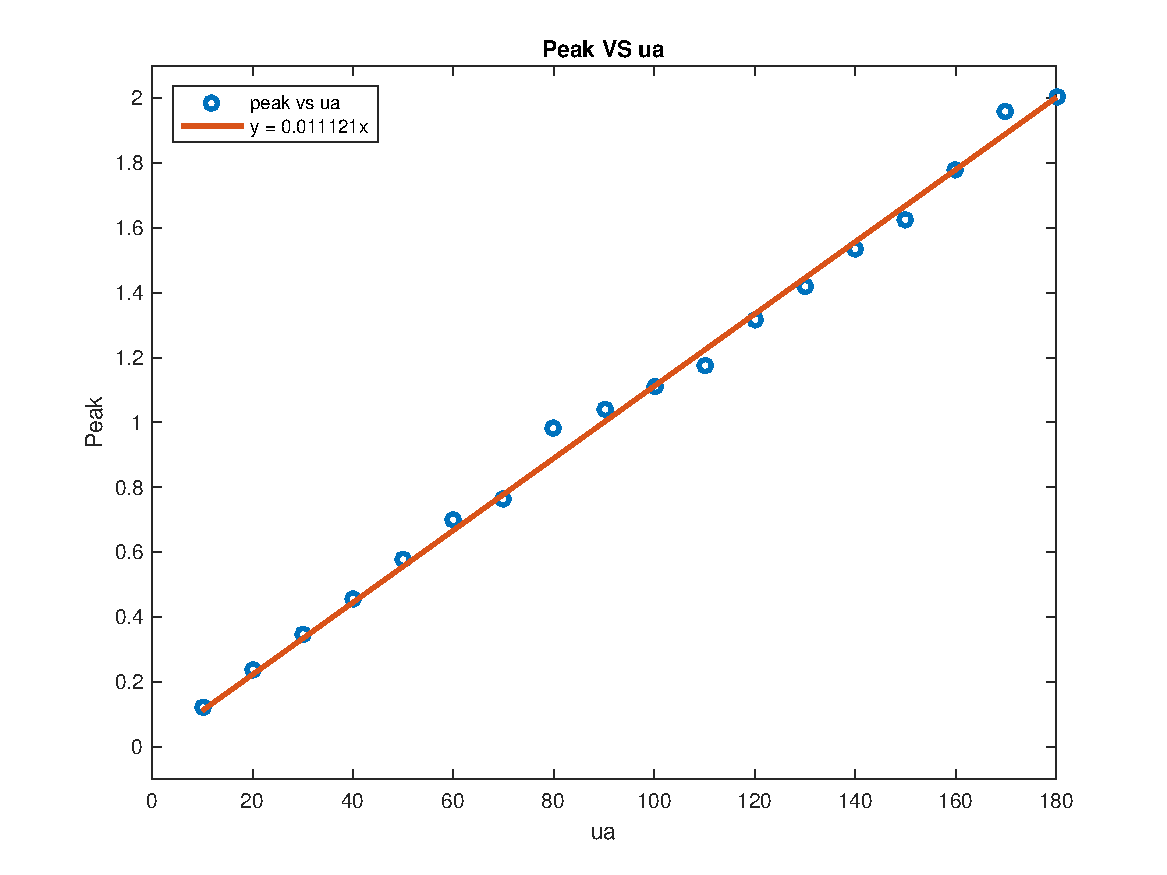
\includegraphics[width=0.7\textwidth]{src/p1d.pdf}
    \caption{peak vs absorbtion coefficient}
    \label{fig:p1d}
\end{figure}
For better visualization, I also plot the curve fitting result for peak and $\mu_a$ and the slope is 0.011 which is very close to
theoretical value 0.0108. So the peak value of noisy signal is still propotional to $\mu_a$.


\subsection{$\mu_a$ (estimated) vs $\mu_a$ (real)}
Similar to Section \ref{sec:p1d}, now for each $\mu_a$ we need to use curve fitting to estimate absorbtion coefficient for them. 
Figure \ref{fig:p1e} shows the result.
\begin{figure}[H]
    \centering
    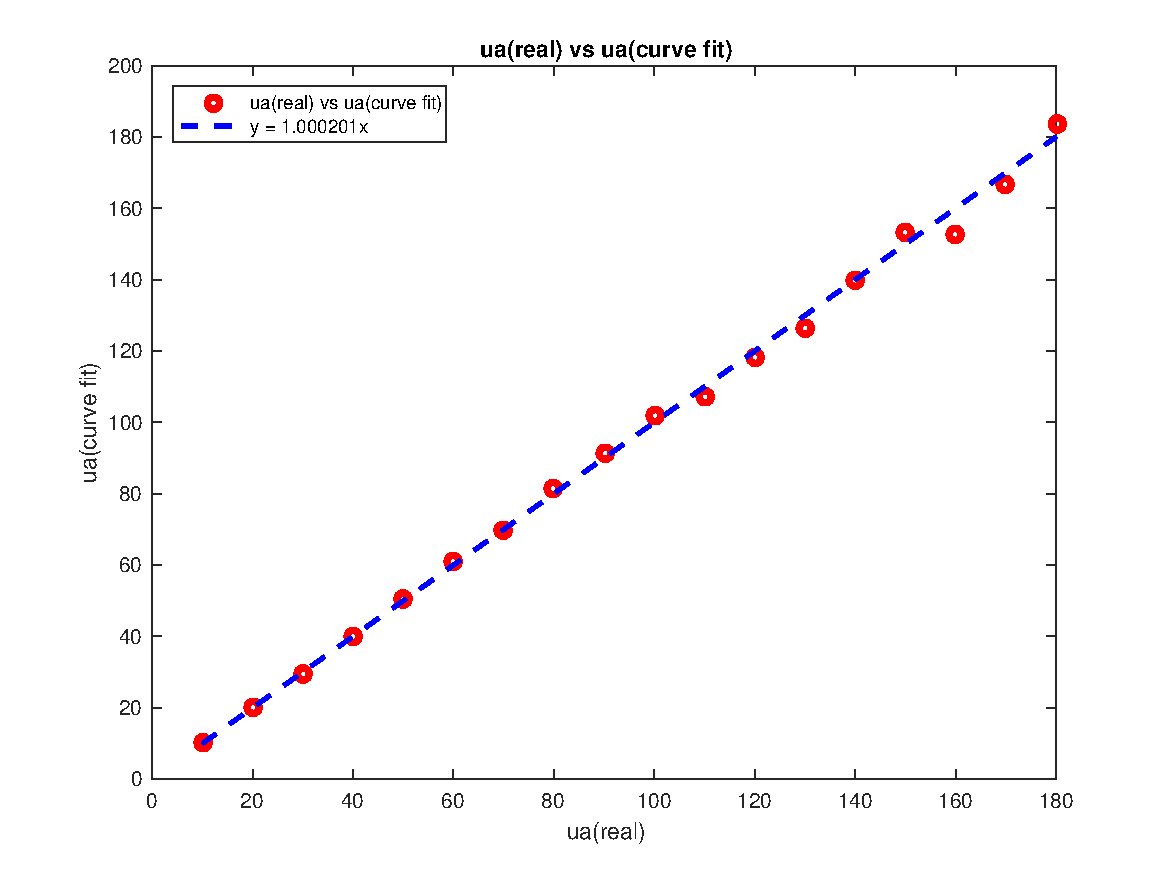
\includegraphics[width=0.7\textwidth]{src/p1e.pdf}
    \caption{$\mu_a$ (estimated) vs $\mu_a$ (real)}
    \label{fig:p1e}
\end{figure}
For better visualization, I use curve fitting for $\mu_a$ (estimated) vs $\mu_a$ (real) in Figure \ref{fig:p1e} and the slope 
is about 1. As a result, our estimated $\mu_a$ is really close to real one.

\subsection{Repeat 4 and 5 with transducer impulse response}
Now we repeat 4 and 5 but considering transducer impulse response. Assume the impulse responses of the transducer used are 
Gaussian pulse centered at 5 MHz, 10 MHz, 25 MHz, and 50 MHz, respectively, with -6 dB fractional bandwidth of 60\%

\subsubsection{Peak value vs absorbtion coefficient}
Figure \ref{fig:p1f-1} show the result of Peak value vs absorbtion coefficient.
\begin{figure}[H]
    \centering
    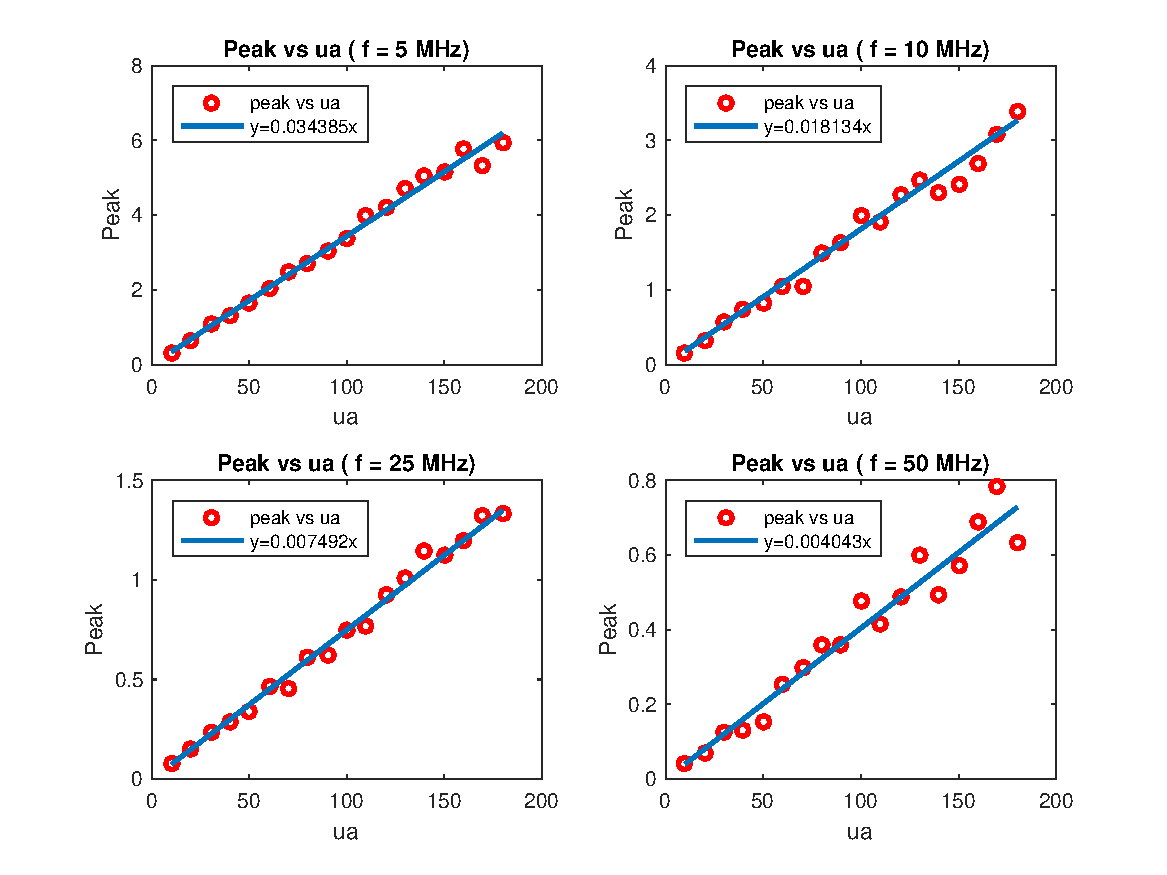
\includegraphics[width=0.9\textwidth]{src/p1f-1.pdf}
    \caption{Peak value vs absorbtion coefficient}
    \label{fig:p1f-1}
\end{figure}
In Figure \ref{fig:p1f-1}, the scalar of between peal and $\mu_a$ is not 0.011. However, we can find that their relation is still 
proportional from the four sub figures. And when center frequecny of transducer become larger, the figure become more noisy

\subsubsection{$\mu_a$ (estimated) vs $\mu_a$ (real)}
Figure \ref{fig:p1f-2} show the result.
\begin{figure}[H]
    \centering
    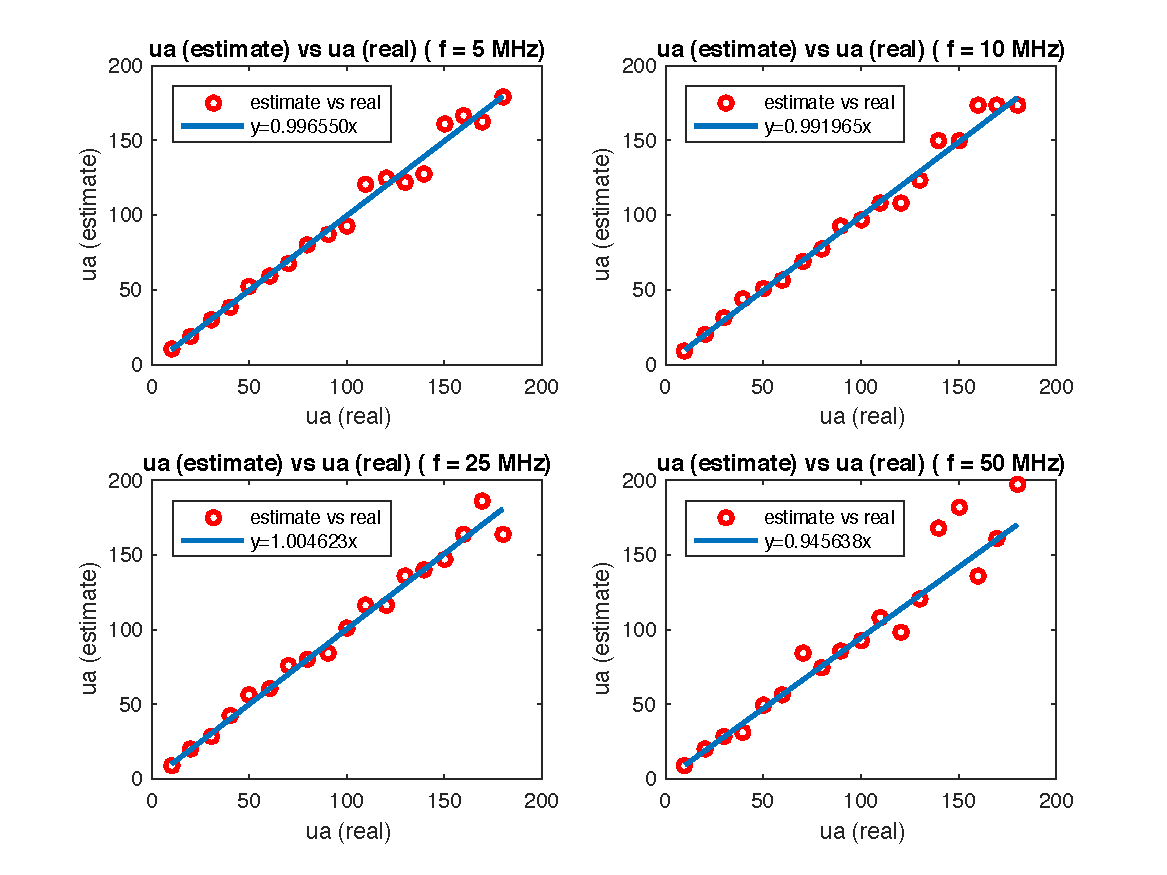
\includegraphics[width=0.9\textwidth]{src/p1f-2.pdf}
    \caption{$\mu_a$ (estimated) vs $\mu_a$ (real)}
    \label{fig:p1f-2}
\end{figure}
In Figure \ref{fig:p1f-2}, we can find that the estimated $\mu_a$ is still close to real $\mu_a$ and the slope is about 1, 
but when transducer center frequency gets larger, the points become much noisier.


\end{document}        
   














